% % % % % % % % % % % % % % % % % % % % % % % % % % % % % % % % % % % % % % % % 
% Formelsammlung von LaTeX4EI									
%
% @encode: 	UTF-8, tabwidth = 4, newline = LF
% @author:	Emanuel Regnath
% @date:		
%
% % % % % % % % % % % % % % % % % % % % % % % % % % % % % % % % % % % % % % % % 


% regex sectionbox(\{([^{]*|(?R))\})
% find (\\sectionbox\{$)  replace \\begin{sectionbox}
% find ^\}$ replace \\end{sectionbox}


%---------------------------------------%
%			P R E A M B L E				%
%~~~~~~~~~~~~~~~~~~~~~~~~~~~~~~~~~~~~~~~%

% Document Class ===============================================================
\documentclass{latex4ei_fs}

\usepackage{colortbl}

\title{System-On-Chip\\Technologies}

\widowpenalty10000

% Dokumentbeginn
% ======================================================================
\begin{document}

\maketitle

% ==============================================================================
\section{General}
% ==============================================================================

\begin{sectionbox}
	\begin{tablebox}{l | ccccccccc}
	$10^\pm$ 	& $21$ & $18$ & $15$ 	&  $12$ & $9$ &  $6$ & $3$ &  $2$ & $1$ \\ \cmrule
	$+$			& $\underset{\ir zetta}{\si{\zetta}}$ & $\underset{\ir exa}{\si{\exa}}$ & $\underset{\ir peta}{\si{\peta}}$	& $\underset{\ir tera}{\si{\tera}}$ & $\underset{\ir giga}{\si{\giga}}$ & $\underset{\ir mega}{\si{\mega}}$ & $\underset{\ir kilo}{\si{\kilo}}$ & $\underset{\ir hecto}{\si{\hecto}}$ & $\underset{\ir deca}{\si{\deca}}$ \\
	$-$ 		& $\underset{\ir zepto}{\si{\zepto}}$ & $\underset{\ir atto}{\si{\atto}}$ & $\underset{\ir femto}{\si{\femto}}$ & $\underset{\ir pico}{\si{\pico}}$ & $\underset{\ir nano}{\si{\nano}}$ & $\underset{\ir micro}{\si{\micro}}$ & $\underset{\ir milli}{\si{\milli}}$  & $\underset{\ir centi}{\si{\centi}}$& $\underset{\ir deci}{\si{\deci}}$
	\end{tablebox}
\end{sectionbox}

% ==============================================================================
\section{SoC Paradigm}
% ==============================================================================


\begin{sectionbox}
    \subsection{Moore's Law}
	Chip capacity (transistors, performance) doubles every 18--24 month
\end{sectionbox}

\begin{sectionbox}
    \subsection{Challenges}
	\textbf{Optimization:} Time-To-Market, Price, Performance, Power Cons.\\
	\textbf{Productivity:} reuse components, shorter development cycles, higher chances for (first time) fault-free
design
\end{sectionbox}

\begin{sectionbox}
    \subsection{Chip Platforms}
	Computation Density (CD) vs Functional Diversity (FD)\\
	\begin{tabular}{@{}l@{\!}llll@{}}
		Platform & CD & FC & units & costs\\ \mrule
		CPU & 40 – 80 & 256 – 16k & ALU\\ 
		DSP & & & Multiplier & very few\\
		ASIP & & & special exec units & few\\
		FPGA & 400 & 1 & LUTs & thousands\\ 
		ASIC & $4\,000$ & 10 & standard cells & millions\\
		Cust. IC & $>\!10\,000$ & $\approx 0$ & transistors & 10 millions\\
	\end{tabular}
	
	\begin{center}
		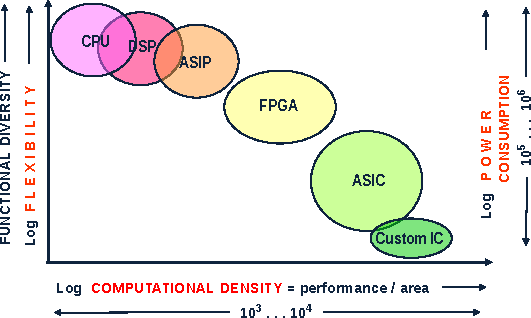
\includegraphics[width = 0.9\columnwidth]{./img/chips.pdf}
	\end{center}
	$CD = \frac{\mathrm{IPC} \cdot f \cdot w \cdot \lambda^2}{A}$\\[0.5em]
	Instructions per cycle IPC, structure size $\lambda$, area $A$\\
	Frequency $f$, Wordsize $w$ (e.g 32 Bit)
\end{sectionbox}


\begin{sectionbox}
	\subsection{CMOS}
	Complementary Metal (Poly-Si) Oxide (SiO2) Semiconductor\\		% temporaly the gate was of Poly-Si, now it is of high-k metal again!
	Why? Low power dissipation, Noise immunity, Clean logic levels, One supply voltage, Cascadable, Easy to design, Fabrication well understood
	%Understand CMOS:\\
	%Electric field at source/channel layer: $\vec E = \frac{V_{\ir gs} - V_{\ir th}}{t_{\ir ox}}$\\
	%Electric field at channel/drain layer:  $\vec E = \frac{V_{\ir gs} - V_{\ir th} - V_{\ir ds}}{t_{\ir ox}}$\\

	%\subsection{Circuits}
		\begin{tabular}{ccc}
			NOT (2 Trans.) & NAND (4 Trans.) & NOR (4 Trans.)\\
			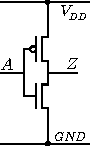
\includegraphics[height = 2cm]{./img/mosfet_not.pdf} \quad & 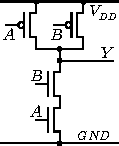
\includegraphics[height = 2cm]{./img/mosfet_nand.pdf} \quad & 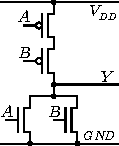
\includegraphics[height = 2cm]{./img/mosfet_nor.pdf} \\
		\end{tabular}
\end{sectionbox}


\begin{sectionbox}
	\subsection{MOSFET}
	\begin{tabular*}{\columnwidth}{@{\extracolsep\fill}lll@{}} \ctrule
		channel width & $W_{\ir n/p}$ \\[0.5em]
		channel length & $L_{\ir n/p}$ \\[0.5em]
		gate oxide thickness & $t_{\ir ox}$ \\[0.5em]
		electron mobility & $\mu_{\ir n} \approx \SI{250e-4}{\meter\squared\per\volt\second}$ \\[0.5em]
		& $\mu_{\ir p} \approx \SI{200e-4}{\meter\squared\per\volt\second}$ \\[0.5em]
		rel. permittivity of gate oxide & $\epsilon_{\ir ox} \approx 3,9$ \\[0.5em]
		dielectric constant & $\epsilon_0 = \SI{8.8541878e-12}{\ampere\second\per\volt\meter}$ \\ \cmrule
		specific oxide capacity & $C'_{\ir ox} = \frac{\varepsilon_{\ir ox} \varepsilon_0}{t_{\ir ox}}$ \\[0.5em]
		oxide capacity & $C_{\ir ox} = C'_{\ir ox} \cdot WL$\\[0.5em]
		gain (also $\beta$) & $K_{\ir n} = \mu_{\ir n} C'_{\ir ox} \frac{W_{\ir n}}{L_{\ir n}}$\\[0.5em]
			& $K_{\ir p} = (-1) \mu_{\ir p} C'_{\ir ox} \frac{W_{\ir p}}{L_{\ir p}}$\\[0.5em]
		propagation delay & $t_{\ir pHL} \propto \frac{C_L t_{\ir ox} L_{\ir p}}{W_{\ir p} \mu_{\ir p} \varepsilon_{\ir ox} (V_{\ir DD} - |V_{\ir th}|)}$ \\
		\cbrule
	\end{tabular*}
\end{sectionbox}






\begin{sectionbox}
	\subsection{Inverter}
	\begin{center}
		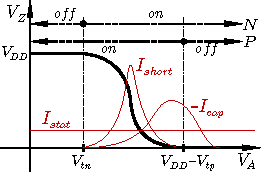
\includegraphics[width = 0.6\columnwidth]{./img/char_inverter.pdf}
	\end{center}
	\begin{tabular}{ll}
		\emph{Dynamic Power Consumption} & $P_{\ir dyn} = P_{\ir cap} + P_{\ir short}$\\
		Capacity Power & $P_{\ir cap} = \alpha_{01} f C_L V_{\ir DD}^2$\\
		Short Circuit Power:	& $P_{\ir short} = \alpha_{01} f \beta_n \tau (V_{\ir DD} - 2V_{\ir th})^3$\\
		%\quad Switching Activity: & $\alpha_{0 \rightarrow 1} = \frac{\text{Schaltvorgänge(pos. Flanke)}}{\text{\# Betrachtete Takte}}$\\
	\end{tabular}\\	
\end{sectionbox}


%\vskip 0em plus 20em minus 0em
%\vbox{
% ==============================================================================
\section{SoC Components}\nopagebreak\par
% ==============================================================================
\makeatletter
 \@afterheading
%\if@nobreak\vspace{5cm}\null\vspace{-5cm}\fi
%\if@nobreak\vfil\vskip-\prevdepth \nointerlineskip\null\penalty 200\vfilneg\fi
\makeatother
%\nobreak
%\ifvmode
%	\penalty 20009
%\else
%	\vadjust{\penalty 20009}
%\fi
%nobreak\par
\begin{sectionbox}
	\subsection{Sequential Logic}
	
	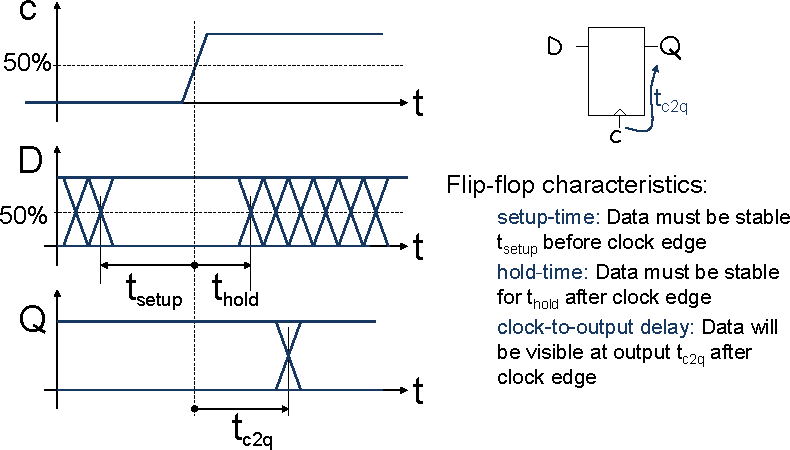
\includegraphics[width = \columnwidth]{./img/timing.pdf}
	
	
	\begin{tablebox}{cc}
			$t_{\ir Setup}$ & setup before clock edge\\
	$t_{\ir hold}$ & hold after clock edge\\
	$t_{\ir c2q}$ & output valid after $t_{\ir c2q}$\\
	Max. clock period &  $t_{\ir clk} \ge t_{1,c2q} + t_{\ir logic,max} + t_{\ir 2,setup}$  \\
	 Max. clockfrequency & $f_{\ir max} = \left\lfloor \frac{1}{t_{\ir clk}} \right\rfloor$ \qquad (Nicht aufrunden) \\
	 hold time condition & $t_{\ir hold} \le t_{\ir c2q} + t_{\ir logic,min}$  $\ra$ Dummy Gate\\
	 Durchsatz & $\frac{1 \text{Sample}}{t_{\ir clk,pipe}} = f$ \\
	 Latenz & $t_{\ir clk} \cdot \#$Pipelinestages (\#FFs - 1) \\
	 Slack & $t_{\ir slack} = t_{\ir available} – t_{\ir required}$\\
	\end{tablebox}
	
	
\end{sectionbox}
%}


\begin{sectionbox}
    \subsection{Karnaugh-Maps}
	\begin{tabular}{l | c | c |  c | r}
	$_z\!\!\diagdown \!\!^{xy}$ & 00 	& 	01	&	11 	&	10	 	\\ \mrule
	0		&	1 \cellcolor{gray!30}	&	0	&	0	&	0		\\	
	1		&	X \cellcolor{gray!30}	&	1 \cellcolor{lightgray}	&	1 \cellcolor{lightgray}	&	0		\\	
	\end{tabular} \hfil
	\parbox{2.5cm}{
	Combine equal cells:\\
	e.g. $\overline x \overline y + y \cdot z$\\
	Use don't care values!}  
		
\end{sectionbox}


\begin{sectionbox}
    \subsection{Finite State Machines}
	\begin{center}
		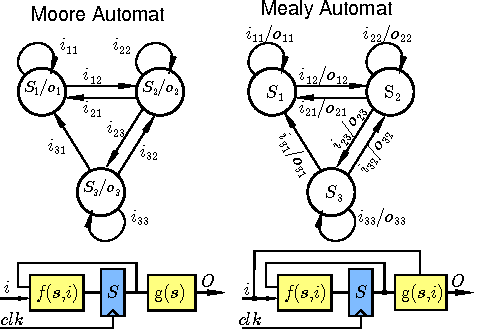
\includegraphics[width = 0.9\columnwidth]{./img/automaten.pdf}
	\end{center}
	Synchronous System Design paradigm: Essentially all control functions in state-of-art digital IC's
	consist of “communicating FSMs”.\\
	Avoid combinatorial logic through paths!\\
	Stick to one FSM design style across SoC!\\ 
\end{sectionbox}


\begin{sectionbox}
    \subsection{Adder}

	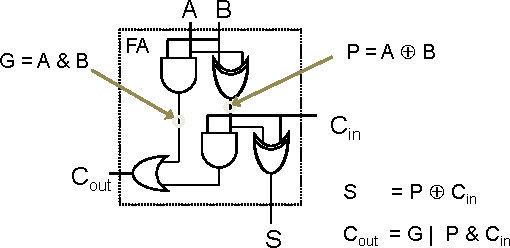
\includegraphics[width = \columnwidth]{./img/fa.pdf}
	
	\subsubsection{Ripple-Carry}
	Worst-Case($G,P = 1$): \qquad  $t_{\ir add} = (N-1) t_{\ir carry} + t_{\ir sum}$\\
	Number of input Bits/Full Adders $N$\\
	
	\subsubsection{Carry-Bypass}
	Fast carry propagation (useful if $N > 4$)\\
	$t_{\ir CBA} = t_{\ir setup} + B t_{\ir carry} + (\frac{N}{B} - 1 ) t_{\ir skip} + (B-1)t_{\ir carry} + t_{\ir sum}$\\
	witch group size in bits $B$.
	$t_{\ir CBA}$ still $\mathcal O(N)$, but with more graduate slope
	
	\subsubsection{Carry-Select}
	Precompute $C_{\ir out}$ for $C_{\ir in} = 0$ and $C_{\ir in} = 1$ for all blocks in parallel.
	Then select the correct one.
	$t_{\ir CSA} = t_{\ir setup} + B t_{\ir carry} + \frac{N}{B} t_{\ir mux} + t_{\ir sum}$\\
	Square Root Carry-Select Adder:\\
	$t_{\ir SCS} = t_{\ir setup} + M t_{\ir carry} + \sqrt{2N}t_{\ir mux} + t_{\ir sum}$\\

\end{sectionbox}


\begin{sectionbox}
    \subsection{Multiplier (Addition of partial products)}
    $x \cdot y = \sum\limits_{j = 0}^{M-1} \sum\limits_{i = 0}^{N-1} x_i y_j \cdot 2^{i+j}$ \quad Result requires $N+M$ bit
    \subsubsection{Repeated Addition}
    
    \subsubsection{Sequential: Right Shift and Add}
    \begin{center}
		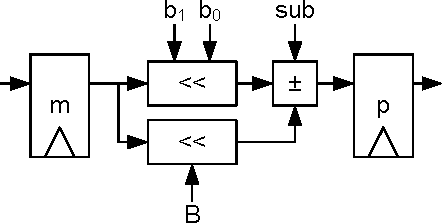
\includegraphics[width = 0.6\columnwidth]{./img/booth_multiplier.pdf}
	\end{center}
    
    \subsubsection{Array Multiplier}
	All partial products generated in
parallel and organized in adder
array with respective offset\\
	$t_{\ir mul} = [(M-1)(N-2)] t_{\ir carry} + (N-1) t_{\ir sum} + t_{\ir and}$
\end{sectionbox}


\begin{sectionbox}
    \subsection{Shifter}
    Single-bit left/ right shift operations through individual pass transistors\\
    Barrel Shifter: Words pass through maximum one transmission gate\\

\end{sectionbox}
\begin{sectionbox}
    \subsection{Multiplexer}
	Mux: $Z = \ol S A_1 + S A_1$ \qquad \quad DeMux: $Z_1 = \ol S A, \quad Z_2 = SA$ 
\end{sectionbox} 

% ==============================================================================
\section{Processor Structure}
% ==============================================================================

\begin{sectionbox}
	\subsection{Processor Classification}
	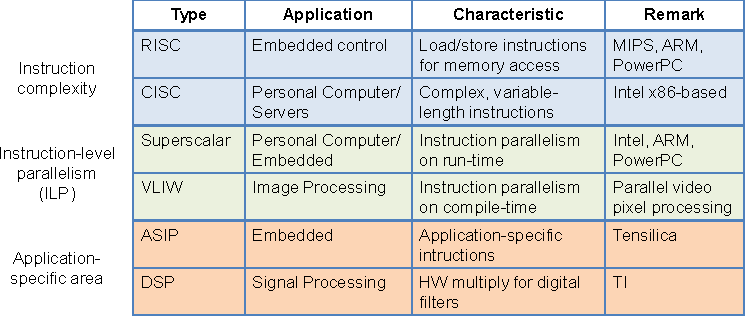
\includegraphics[width = \columnwidth]{./img/cpus}
\end{sectionbox}

\begin{sectionbox}
	\subsection{Software Levels}
	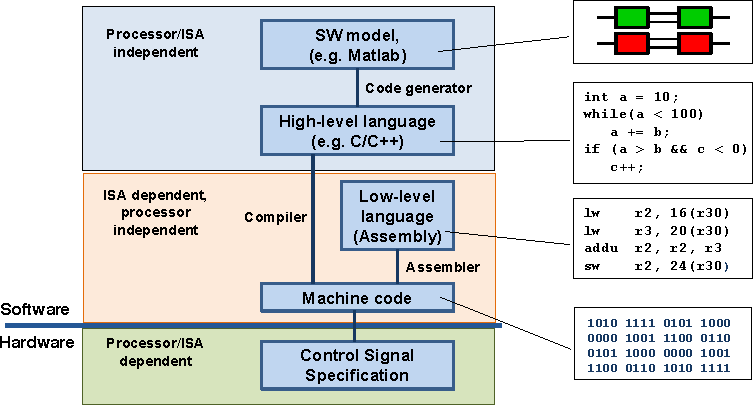
\includegraphics[width = \columnwidth]{./img/swlevels}
\end{sectionbox}


\begin{sectionbox}
	\subsection{Multi Cycle Core}
	\begin{description}
		\item[1. Instruction Fetch (IF):] increase PC
		\item[2. Instruction Decode (ID):] read OP and register
		\item[3. Execution (EX):] ALU executes command
		\item[4. Memory Stage (M):] read/write to memory
		\item[5. Write Back (WB):] load from memory to register?
	\end{description}	
\end{sectionbox}


\begin{sectionbox}
    \subsection{Hazards (problems due to pipelining)}
	\textbf{Structural Hazard:} same resource is needed multiple times in the same cycle\\
		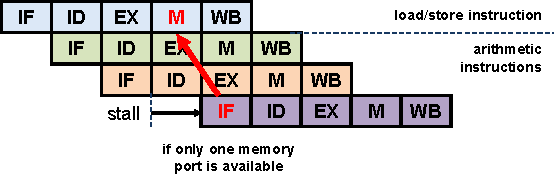
\includegraphics[width = 0.9\columnwidth]{./img/hazard_structural}\\
	\\
	\textbf{Data Hazard:} data dependencies (read-after write, write-after-write, write-after-read).\\
		Solution: Forwarding, Stalling, Scheduling\\
		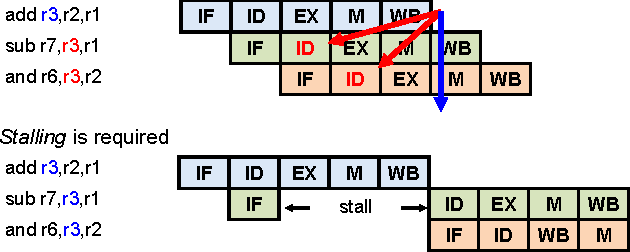
\includegraphics[width = \columnwidth]{./img/hazard_data}\\
		With register forwarding: Only 1 stall below EX.\\ 
	\\
	\textbf{Control Hazard:} next executed instruction is not the next specified instruction due to jump, branch, exception.\\
		Solution: Branch prediciton\\
		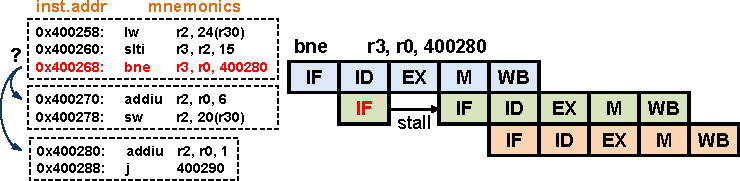
\includegraphics[width = \columnwidth]{./img/hazard_control}\\
\end{sectionbox}


\begin{sectionbox}
    \subsection{Processor Performance}
	$\mathrm{CPU Time} = \underbrace{\frac{\mathrm{Instructions}}{\mathrm{Program}}}_{\mathrm{Estimate}} \cdot \underbrace{\frac{\mathrm{Clock Cycles}}{\mathrm{Instruction}}}_{\mathrm{CPI}}  \cdot \underbrace{\frac{\mathrm{Seconds}}{\mathrm{Clock Cycle}}}_{\frac{1}{f_{\ir CPU}}}$
\end{sectionbox}








% ==============================================================================
\section{Memory}
% ==============================================================================

\newcommand{\twocell}[2]{\vtop{\hbox{\strut #1}\hbox{\strut #2}}}
\newcommand{\multicell}[2][t]{\begin{tabular}[#1]{@{}l@{}}#2\end{tabular}}

\begin{sectionbox}
	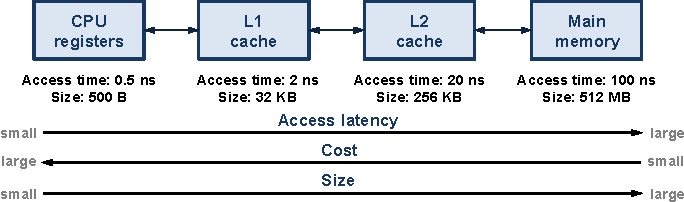
\includegraphics[width = \columnwidth]{./img/memory_hierarchy}
	\renewcommand{\arraystretch}{1.5}
	\begin{tablebox}{llll} 
		\textbf{Type} & \textbf{Used} & \textbf{Speed} & \textbf{Density}\\ \cmrule
		Register & \twocell{CPU Registers}{$32 \cdot \SI{64}{bit}$} & $< \si{ns}$ & \\
		On-Chip SRAM & \twocell{Cache}{$\SI{32}{kByte}$} & $\si{ns}$ & \\[0.5em]
		DDR3 SDRAM & \twocell{Main Memory}{$\approx \si{GByte}$} & $2 \cdot \SI{800}{MHz}$ & \\
		HDD & \twocell{Mass Storage}{$> \si{TB}$} & $150 \frac{\si{MB}}{\si{s}}$\\
		ROM & \twocell{Sys. Config}{few $\si{kByte}$} & $\approx \si{kB \per s}$\\
	\end{tablebox}
\end{sectionbox}





\begin{sectionbox}
	\subsection{CMOS Memory}
	Register: 2 Inverters (Q,$\ol{\text{Q}}$)\\
	Latch: 4 NANDS (e,D,Q,$\ol{\text{Q}}$)\\
	Flip-Flop: (Q,$\ol{\text{Q}}$, clk)\\
\end{sectionbox}


\begin{sectionbox}
    \subsection{Cache}
    Caches store only small share of main memory. The Cache maps RAM-Addresses to Cache-Entries. One Cache-Entry can contain several Data Bytes. The Tag verifies the mapping, the Valid-Flag verifies the actuality of the cached data.\\
    
    \begin{tablebox*}{lll}
		RAM-Address & & RAM-Data\\
		\framebox{\strut Tag---Index---Offset} & $\ra$ & \framebox{\strut Data}\\[1em]
		Cache-Address & & Cache-Entry\\
		\framebox{\strut Index} & $\ra$ & \framebox{\strut Flags---Tag---Data}\\
	\end{tablebox*}
	
	\#RAMAddressBits = \#TagBits + \#IndexBits + \#OffsetBits\\
	\#CacheEntries = $2^{\ir Indexbits}$\\
	\#CacheDataBytes = $2^{\ir Offsetbits}$ \qquad (Byte accurate Cache access)\\
	CacheSizeInByte = \#CacheEntries $\cdot$ \#CacheDataBytes\\
	

	\subsubsection{Direct Mapped Cache}
	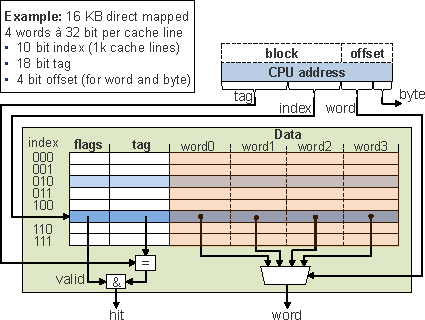
\includegraphics[width = \columnwidth]{cache_direct}

	Replace Strategy: Replace old with new.

	\subsubsection{Set-Associative-Cache}
	Blocks with equal Index can be stored in $n$ cache entries. Tag needed to distinguish.
	Replace Strategy: Replace if all sets are full. Random, FIFO or LRU (least recently used)\\
	$\frac{\text{\#Zugriffe}}{\text{Zeit}} = \text{Hit-Rate} \cdot \text{Hit-Time} + \text{Miss-Rate} \cdot \text{Miss-Time}$ \\

	\subsubsection{Fully Associative Cache}
	A memory block can be stored in any cache entry.
\end{sectionbox}


\begin{sectionbox}
    \subsection{Branch Prediction}
    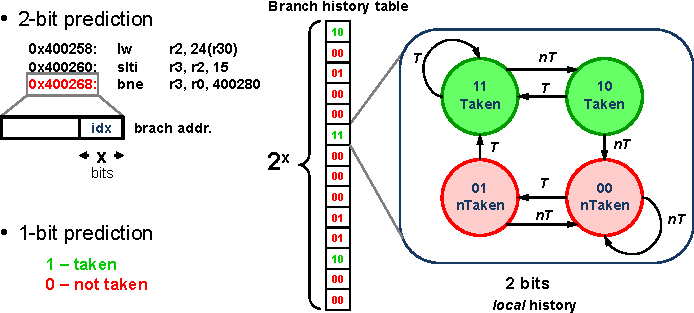
\includegraphics[width = \columnwidth]{branch_prediction}
    
\end{sectionbox}


\begin{sectionbox}
	\subsection{Main Memory}
	
	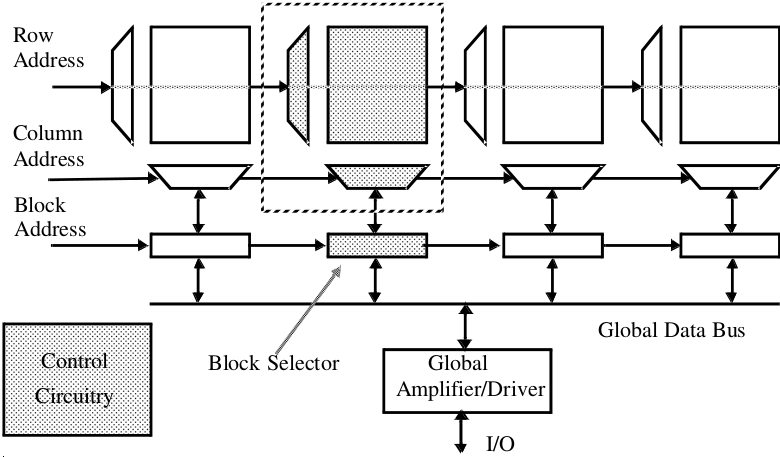
\includegraphics[width = \columnwidth]{./img/memory}
	
	$ΔV = (V_X - V_{\ir Pre}) \cdot \frac{C_{\ir S}}{C_{\ir S} + C_{\ir BL}}$	\qquad $V_{\ir Pre} \approx 0.5 V_{\ir DD}$\\
	$ΔV_{\ir BL} = V_{\ir eq} - V_{\ir BL} = \pm \frac{C_{\ir S}}{C_{\ir S} + C_{\ir BL}} \cdot \frac{V_{\ir DD}}{2}$\\
	
	\subsection{Memory Block}
	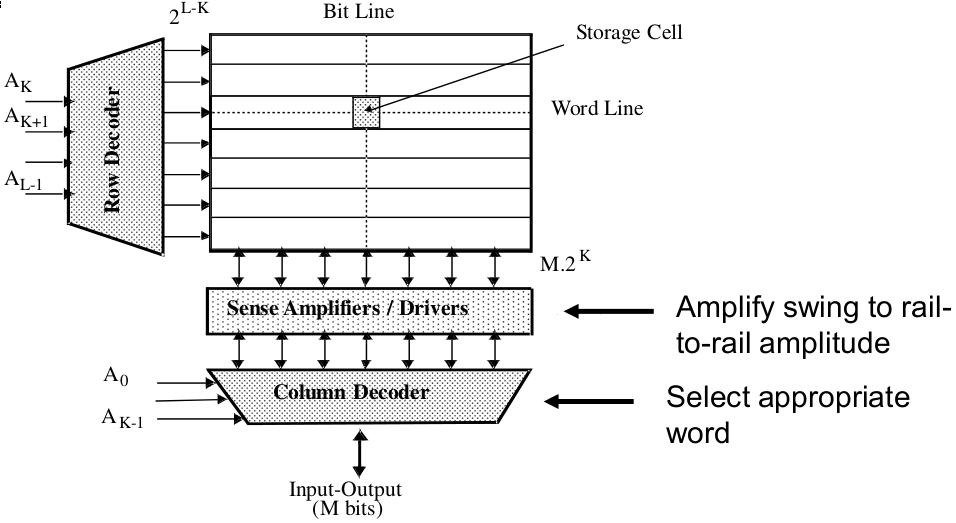
\includegraphics[width = \columnwidth]{memory_block}
	
	
	\subsection{Memory cell types} 
	\begin{tabular*}{\columnwidth}{@{\extracolsep\fill}ll@{}} \ctrule
		\large \bf DRAM & \large \bf SRAM \\ 
		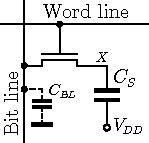
\includegraphics[width = 1.9cm]{./img/DRAM} & 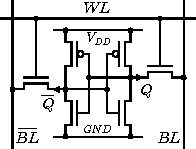
\includegraphics[width = 2.6cm]{./img/SRAM} \\[2em]
		\large \bf Flash & \large \bf ROM \\
		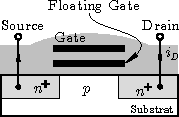
\includegraphics[width = 2.5cm]{./img/flash} & 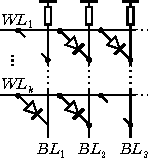
\includegraphics[width = 1.8cm]{./img/ROM}\\ \cbrule
	\end{tabular*}
	
	DRAM Timings: $t_{\ir CAS}$--$t_{\ir RCD}$--$t_{\ir RP}$--$t_{\ir RAS}$\\
	Access Latency: $t_{\ir Lat} = t_{\ir CAS} + t_{\ir RCD}$\\
	Min. row cycle: $t_{\ir RC} = t_{\ir RP} + t_{\ir RAS}$\\
	
	%Transfer Rate: $TR =  
	
	Access Times:\\
	\begin{tabular}{lll}
	DRAM: & Single: & (cLatency + 1c(amp)) $\cdot$ \#reads\\
		& Burst: & cLatency + (\#reads-1) + 1c(amp)\\
	SRAM & Single: & cLatency $\cdot$ \#reads\\
		& Burst: & cLatency + (\#reads-1)
	\end{tabular}
\end{sectionbox}






\columnbreak

% ==============================================================================
\section{Interconnect}
% ==============================================================================


\begin{sectionbox}
	\subsection{Interconnection}
	
	\subsubsection{Processor Local Bus (PLB)}
	Bus-Transaction: Request $\ra$ Addr. Trans. $\ra$ Data Trans.$\ra$ Data Ack\\
	Burst Transfer: Reduction of Req./Addr. signaling overhead for read/ write
transactions to consecutive addresses. Burst transfers with implicit address increment\\

	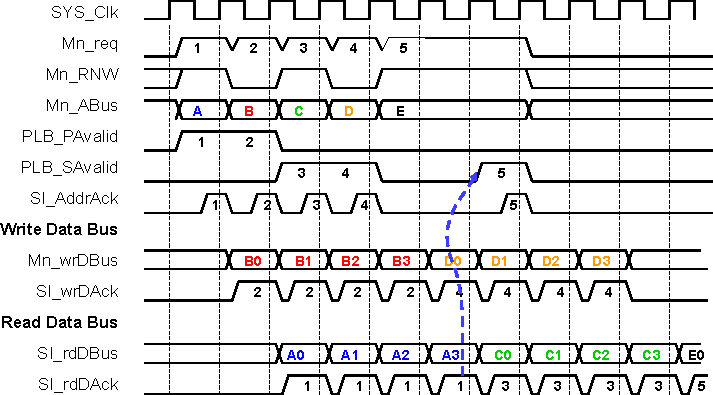
\includegraphics[width = \columnwidth]{./img/interconnect_bus}

\end{sectionbox}


\begin{sectionbox}
	Bus Standard: AMBA (ARM), CoreConnect (IBM), OCP (Sonics), VSIA\\
	\subsection{AMBA AHB}
	\textbf{A}dvanced \textbf{M}icrocontroller \textbf{B}us \textbf{A}rchitecture
	\textbf{A}dvanced e\textbf{X}tensible \textbf{I}nterface
\end{sectionbox}


\begin{sectionbox}
	\subsection{FIFOs}
	Are use for decoupling clock domains or word widths.\\
	Pointer: Read (RP) and Write (WP)\\
	Control Flags: Almost Full (AF) and almost empty (AE)

\end{sectionbox}

\begin{sectionbox}
	\subsection{Network-on-Chips (NoC)}
	Benefits: Scalability, Synchronization, short point-to-point links\\
	Drawbacks: Latency, Area
\end{sectionbox}

% ==============================================================================
\section{Low Power Design}
% ==============================================================================


\begin{sectionbox}
	\subsection{Motivation -- Why?}
	\begin{itemize}
		\item Reliability: Plus 10$^\circ$C doubles failure rate
		\item High currents destroy on-chip wires
		\item Cooling: higher costs and power consumption
	\end{itemize}
	
	Leakage current: $I_{\ir leak} \propto \exp(V_{\ir GS} - V_{\ir th})$\\
	Gate Delay: $t_{\ir d} \propto \frac{C_L}{V_{\ir DD} - V_{\ir th}}$
\end{sectionbox}


\begin{sectionbox}
	\subsection{Techniques and Hierarchy}
	Trade in Power with Performance, Area, Cost\\
	\\
	Frequency Scaling and Voltage Scaling (DFS, DVS) \\
	Algorithmic Optimization: $x^2 + ax = x(x+a)$\\
	Power Gating: Switch components off if not needed.\\
	\textbf{Clock Gating:} toggle registers only when outputs can change\\
	Threshold Control: bias threshold voltage $V_{\ir th}$
\end{sectionbox}






% Dokumentende
% ======================================================================
\end{document}

\columnbreak


{\huge\bf Tutorials}

\begin{sectionbox}
	\subsection{Introduction}
	
		\subsubsection{Ex1}
			Left-Right, Top-Bottom: A,B,D,-  
	
		\subsubsection{Ex2}
			a) Propagation Delay $t_{PLH} \propto \frac{C t_{\ir ox} L_p}{W_p \mu_p \varepsilon (V_{\ir dd} - V_{\ir thp})}$\\
			If $W_p$ is increased, $C$ will also increase and compensate!\\
			b) $A = \uparrow W \cdot L$			% bigger area -> higher probability of broken chips
				Power $P$ 
			
			c)
\end{sectionbox}

\begin{sectionbox}
	\subsection{SoC Paradigm}

		\subsubsection{Ex1}
			b) CPU: $CD = \frac{performance}{area} = \frac{2 \cdot 32 op \cdot \SI{466}{MHz}}{\frac{9mm^2}{(\SI{110}{nm})^2}} = 40 \frac{\si{op}}{\si{s sq}}$\\
			c) possible reasons: cahce misses + DRAM latencies\\
			d) ASIP: $CD = \frac{2 \cdot \SI{311}{MHz}}{\frac{0.45}{110^2}} = 268 \frac{\si{op}}{\si{s sq}}$\\
			e) FPGA: $CD = \frac{3333 \cdot \SI{200}{MHz}}{\frac{\SI{7}{mm\squared}}{(\SI{70}{nm})^2}} = 467 \frac{\si{op}}{\si{s sq}}$\\
			f) ASIC: $CD = \frac{1 \cdot \frac{1}{\SI{0.43}{ns}}}{\frac{\SI{90}{\micro\meter\squared}}{(\SI{70}{nm})^2}} = 127 \frac{\si{kop}}{\si{s sq}}$\\

		\subsubsection{Ex2}
		$T = 1000 + (100+400+700+100)\cdot\frac{16}{N} + 1000$\\
		b) Single Core: $f=1824 Mhz$\\
		d) $T=2000+\frac{20800}{4} = 7200$, $f=576 Mhz$\\

		Lower frequency $\to$ allows higher propagation delay $\to$ allows lower voltage\\
		$P_{\ir dyn} \propto f \cdot V_{\ir dd}^2$\\
		$P_{\ir multi} = \frac{f}{k} \left( \frac{V_{\ir dd}}{k} \right)^2 n$ \qquad $k = \frac{1824}{516} = 3.17$\\ 
		$P_{\ir multi} = 0.13 \cdot P_{\ir single}$ for Quadcore!\\ 
\end{sectionbox}



\begin{sectionbox}
	\subsection{SoC Component Design}

		\subsubsection{Exercise 1}
		

\end{sectionbox}


\begin{sectionbox}
	\subsection{Finite State Machines}
	

		\subsubsection{Exercise 4}
		a) 1,0,0,out=1 := 4 states\\ 
		b) 1/0, 0/0, 0/0 := 3 states\\
		c) Table with $x_1,x_0,A,N_1,N_0$\\

	$t_{clk} = t_{c2q} + t_{logic} + t_{setup} = 100 + 6120 + 150 = \SI{6370}{\pico\second}$\\
	Mealy FSM: $t = 150 + 4000 + 140 + 6000 + 100$ \qquad $\SI{96.2}{\mega\hertz}$\\
	$f_{clk} = 1/t_{clk} = $
\end{sectionbox}


\begin{sectionbox}
	\subsection{Processor Pipeline}
	a) NoPipelining: Cycles Per Instruction: 5 because: F,D,E,M,W\\
	b) Pipelingin: Hazard: wait 4 cycles in Decode, Writeback must be finished before Decode starts\\
		No Branch Prediction, Fetch can only start after execution is finished. CPI = 21/10 = 2.1\\
	c) Register Forwarding: 2 cycles in Decode because previous result valid after execution. CPI = 15/10 = 1.5\\


\end{sectionbox}


\begin{sectionbox}
	\subsection{Generic Model of Static CMOS}
In general, a generic model can be used to convert Boolean equations into static
CMOS circuits. Each AND function generates serially connected nMOS transistors
on a path from the output to GND, complemented by parallel connected pMOS tran-
sistors on a path from the output to VDD. Each OR function generates parallel
nMOS, complemented by serial pMOS transistors, respectively. Finally, the output is
always inverted, due to the switching properties of MOS transistors.
\end{sectionbox}

A variety of microprocessor architectures in embedded systems
Instruction Set Architecture as interface between hardware
and software
Performance is limited mainly by memory access, code
parallelism and data dependencies
